\chapter{Complex Manifolds}
\section{Remaining Problems Of Reading}
\subsection{The Expression of the Fundamental Form}
1. By definition of $(~ ,~ )$, i.e. $(~,~) := \langle ~,~\rangle-i\cdot \omega$, one has $\omega=-\Im( , )$ and $\langle , \rangle=\Re( , )$. Hence,
\begin{subequations}\label{w expression}
  \begin{align}
\omega(x_i,x_j) =\omega(y_i,y_j) &=-\Im(h_{ij}),\\
\omega(x_i,y_j) &=\Re(h_{ij}),\\
\langle x_i ,x_j\rangle =\langle y_i,y_j\rangle &=\Re(h_{ij}),\\
\langle x_i,y_j\rangle &=\Im(h_{ij}).
\end{align}
\end{subequations}
Thus
\[
  \omega=-\sum_{i<j} \Im(h_{ij})(x^i\wedge x^j+y^i\wedge y^j )+\sum_{i,j=1}^{n}\Re(h_{ij})x^i\wedge y^j.
\]
\begin{proof}
  Let Hermite structure be written as $H(x,y)=F(x,y)+iG(x,y)$. where $F(x,y)$ is  real value bilinear symmetry function and $G(x,y)$ is  real value bilinear anti-symmetry function. Then the fundamental form $\omega=\widehat{H}(x,y)$ can be expressed as the form
  \begin{align*}
    G(x,y) &=-\frac{i}{2}(H(x,y)-\overline{H(x,y)})\\
    &=-\frac{i}{2}\sum_{j,k} h_{j\overline{k}} (\lambda^j(x)\overline{\lambda^k}(y)-\lambda^j (y)\overline{\lambda^k}(x))\\
    &=-\left\langle x\wedge y,\frac{i}{2}\sum h_{j\overline{k}} \lambda^j\wedge\overline{\lambda^k}\right\rangle,
  \end{align*}
  As 
  \[
    \langle x\wedge y, \widehat{H}\rangle=-G(x,y),
  \]
  thus 
  \[
    \omega=\widehat{H}=\frac{i}{2}h_{j\overline{k}} \lambda^j\wedge\overline{\lambda^k}\in \Wedge[2] V^*\cap \Wedge[1,1] V^*.
  \]
    Then let $\lambda^s=x^s+i y^s, s=j,k$, a calculation yields the conclusion\cite{LDG}.
\end{proof}
\Line
2. Using an orthogonal basis $x_1,y_1=I(x_1), \cdots, x_n,y_n=I(x_n)$, we have 
\[
  n!\cdot \omega^n=\mathrm{vol}.
\]
\begin{proof}
  \begin{align*}
 \omega^n&=\bigl(\sum_{i=1}^{n}x^i\wedge y^i\bigr)^n\\
 &=\underbrace{\bigl(\sum_{i=1}^{n}x^i\wedge y^i\bigr)\wedge \bigl(\sum_{i=1}^{n}x^i\wedge y^i\bigr)\cdots\wedge \bigl(\sum_{i=1}^{n}x^i\wedge y^i\bigr)}_{n}\\
 &=\sum_{i_1,i_2,\cdots,i_n=1}^n (x^{i_1}\wedge y^{i_1})\wedge (x^{i_2}\wedge y^{i_2})\wedge\cdots (x^{i_n}\wedge y^{i_n})\\
 &=\frac{1}{n!} (x^1\wedge y^1)\wedge (x^2\wedge y^2)\wedge \cdots (x^n\wedge y^n)\\
 &=\frac{1}{n!}\cdot \mathrm{vol}.
  \end{align*}
  ,where items that are not naturally arranged (i.e. $i_1,i_2,\cdots,i_n$) can always be changed into a natural arrangement by swapping them with an even number of inversions i.e. theirs coefficients can be written as $(-1)^{2\cdot m}$.
\end{proof}
\Line
\section{Complex and Hermitian Structure}
\begin{definition}[][\textit{\textbf{Lefschetz Operator $L$}}]
   Let $(V,\langle~,~\rangle) $ be an euclidian vector space and let $I$ be a compatible almost complex structure. Furthermore, let $\omega$ be the associated fundamental form. Then the \textsf{Lefschetz operator} $L: \bigwedge^* V_{\mathbb{C}}^* \rightarrow \bigwedge^* V_{\mathbb{C}}^*$ is given by $\alpha \mapsto \omega \wedge \alpha$.
\end{definition}
\begin{remark}
The following properties are easy to verify:

i) $L$ is the $\mathbb{C}$-linear extension of the real operator $\bigwedge^* V^* \rightarrow \bigwedge^* V^*;  \alpha \mapsto \omega \wedge \alpha$.

ii) The Lefschetz operator is of bidegree $(1,1)$, i.e.
$$
L\bigl(\Wedge[p, q] V^*\bigr) \subset \Wedge[p+1, q+1] V^*
$$
Furthermore the Lefschetz operator induces bi jections
$$
L^k: \Wedge[k] V^* \stackrel{\simeq}{\longrightarrow} \Wedge[2n-k] V^*
$$
\end{remark}

\begin{definition}[][\textit{\textbf{Hodge $*$--operator}}]
  The \textsf{Hodge $*$--operator} is difined by 
\[
  \alpha\wedge*\beta=\langle\alpha,\beta\rangle\cdot \mathrm{vol}.
\]
for $\alpha,\beta\in \bigwedge^* V$. This determines $*$ , for exterior product defines a nondegenerate pairing $\bigwedge^k V\times \bigwedge^{d-k} V\to \bigwedge^d V=\mathrm{vol}\cdot \bR$. One easily sees that $*\colon \bigwedge^k V\to \bigwedge^{d-k} V$.
\end{definition}

\begin{proposition}
  Let $(V,\langle~,~\rangle)$ be an oriented euclidian vector space of dimension d. Let $e_1, \ldots, e_d$ be an orthonormal basis of $V$ and let $\mathrm{vol} \in \bigwedge^d V$ be the orientation of norm one given by $e_1 \wedge \ldots \wedge e_d$. The Hodge $*$-operator associated to $(V,\langle~,~\rangle, \mathrm{vol})$ satisfies the following conditions:
\begin{enumerate}[label=\roman*),font=\upshape]
  \item If $\left\{i_1, \ldots, i_k, j_1, \ldots, j_{d-k}\right\}=\{1, \ldots d\}$ one has
$$
*\left(e_{i_1} \wedge \ldots \wedge e_{i_k}\right)=\varepsilon \cdot e_{j_1} \wedge \ldots \wedge e_{j_{d-k}},
$$
where $\varepsilon=\operatorname{sgn}\left(i_1, \ldots, i_k, j_1 \ldots j_{d-k}\right)$. In particular, $* 1= \mathrm{vol}$.
  \item The *-operator is self-adjoint up to sign: For $\alpha \in \bigwedge^k V$ one has
$$
\langle\alpha, * \beta\rangle=(-1)^{k(d-k)}\langle * \alpha, \beta\rangle .
$$
  \item The *-operator is involutive up to sign:
$$
\left(* \big|_{\wedge^k V}\right)^2=(-1)^{k(d-k)}
$$
  \item The Hodge *-operator is an isometry on $\left(\bigwedge^* V,\langle~,~\rangle\right)$.
\end{enumerate}
\end{proposition}
\begin{definition}[][\textbf{\textit{Dual Lefschetz Operator $\Lambda$}}]
  The \textsf{dual Lefschetz operator} $\Lambda$ is the operator $\Lambda\colon \bigwedge^* V^*\to\bigwedge^* V^*$ that is \textbf{\textit{adjoint}} to $L$ with respect to $\langle~,~\rangle$, i.e. $\Lambda\alpha$ is uniquely determined by the condition 
  \[
    \langle \Lambda\alpha,\beta\rangle=\langle\alpha,L\beta\rangle, \quad \text{for all} ~\beta\in \Wedge[*]V^*.
  \]
\end{definition}
\clearpage
\begin{proposition}
  The dual Lefschetz operator $\Lambda$ is of degree $-2$ , i.e. 
  $$\Lambda\bigl(\Wedge[k] V^*\bigr) \subset\Wedge[k-2] V^*.$$ 
  Moreover, one has $\Lambda=*^{-1} \circ L \circ *$.
\end{proposition}
\begin{proof}
The first assertion follows from the fact that $L$ is of degree $2$ and that $\bigwedge^* V^*=\bigoplus \bigwedge^k V^*$ is orthogonal.

By definition of the Hodge $*$-operator one has $\langle\alpha, L \beta\rangle \cdot \mathrm{vol}=\langle L \beta, \alpha\rangle \cdot \mathrm{vol}=$ $L \beta \wedge * \alpha=\omega \wedge \beta \wedge * \alpha=\beta \wedge(\omega \wedge * \alpha)=\left\langle\beta, *^{-1}(L(* \alpha))\right\rangle \cdot\mathrm{vol}$.
\end{proof}
\begin{lemma}
  Let $\langle,\rangle_{\mathbb{C}}, \Lambda$, and $*$ be as above. Then
  \begin{enumerate}[label=\roman*),font=\upshape]
    \item The decomposition $\bigwedge^k V_{\mathbb{C}}^*=\bigoplus \Lambda^{p, q} V^*$ is orthogonal with respect to $\langle,\rangle_{\mathbb{C}}$.
    \item The Hodge *-operator maps $\bigwedge^{p, q} V^*$ to $\bigwedge^{n-q, n-p} V^*$, where $n=$ $\operatorname{dim}_{\mathbb{C}}(V, I)$.
    \item $\bullet$ The dual Lefschetz operator $\Lambda$ is of bidegree $(-1,-1)$, i.e. 
    $$\Lambda\Bigl(\Wedge[p, q] V^*\Bigr) \subset\Lambda^{p-1, q-1} V^*.$$
  \end{enumerate}
\end{lemma}
\begin{definition}[][\textit{\textbf{Counting Operator $H$}}]
  Let $H\colon \Wedge[*]V\to\Wedge[*]V$ be the \textsf{counting operator} defined by $H|_{\bigwedge^k V}=(k-n)\cdot \mathrm{id}$, where $\dim_{\bR}V=2n$. Equivalently, 
  \[
    H=\sum_{k=0}^{2n}(k-n)\cdot \prod\nolimits^k.
  \]
\end{definition}
\begin{proposition}[][][prop: comutators]
  Let $(V,\langle~,~\rangle)$ be an euclidian vector space endowed with a compatible almost complex structure I. Consider the following linear operators on $\bigwedge^* V^*$ : The associated Lefschetz operator $L$, its dual $\Lambda$, and the counting operator $H$. They satisfy:
  \begin{center}
    i) $[H, L]=2 L$, \quad ii) $[H, \Lambda]=-2 \Lambda$, \quad and \; iii) $[L, \Lambda]=H$.
  \end{center}
\end{proposition}

\begin{proof}
  Let $\alpha \in \bigwedge^k V^*$. Then $[H, L](\alpha)=(k+2-n)(\omega \wedge \alpha)-\omega \wedge((k-n) \alpha)=$ $2 \omega \wedge \alpha$. Analogously, $[H, \Lambda](\alpha)=(k-2-n)(\Lambda \alpha)-\Lambda((k-n) \alpha)=-2 \Lambda \alpha$.
  
The third assertion is the most difficult one. We will prove it by induction on the dimension of $V$. Assume we have a decomposition $V=W_1 \oplus W_2$ which is compatible with the scalar product and the almost complex structure, i.e. $(V,\langle~,~\rangle, I)=,\left(W_1,\langle~,~\rangle_1 , I_1\right) \oplus\left(W_2,\langle~,~\rangle_2, I_2\right)$. Then $\bigwedge^* V^*=\bigwedge^* W_1^* \otimes \bigwedge^* W_2^*$ and in particular $\bigwedge^2 V^*=\bigwedge^2 W_1^* \oplus \bigwedge^2 W_2^* \oplus W_1^* \otimes W_2^*$. Since $V=W_1 \oplus W_2$ is orthogonal, the fundamental form $\omega$ on $V$ decomposes as $\omega_1 \oplus \omega_2$, where $\omega_i$ is the fundamental form on $W_i$ (no component in $W_1^* \otimes W_2^*$ ). Hence the Lefschetz operator $L$ on $\bigwedge^* V^*$ is the direct sum of the Lefschetz operators $L_1$ and $L_2$ acting on $\bigwedge^* W_1^*$ and $\bigwedge^* W_2^*$, respectively, i.e. $L=L_1+L_2$ with $L_1$ and $L_2$ acting as $L_1 \otimes 1$ respectively $1 \otimes L_2$ on $\bigwedge^* W_1^* \otimes \bigwedge^* W_2^*$.

Let $\alpha, \beta \in \bigwedge^* V^*$ and suppose that both are split, i.e. $\alpha=\alpha_1 \otimes \alpha_2$, $\beta=\beta_1 \otimes \beta_2$, with $\alpha_i, \beta_i \in \bigwedge^* W_i^*$. Then $\langle\alpha, \beta\rangle=\left\langle\alpha_1, \beta_1\right\rangle \cdot\left\langle\alpha_2, \beta_2\right\rangle$. Therefore,
$$
\begin{aligned}
\langle\alpha, L \beta\rangle & =\left\langle\alpha, L_1\left(\beta_1\right) \otimes \beta_2\right\rangle+\left\langle\alpha, \beta_1 \otimes L_2\left(\beta_2\right)\right\rangle \\
& =\left\langle\alpha_1, L_1 \beta_1\right\rangle\left\langle\alpha_2, \beta_2\right\rangle+\left\langle\alpha_1, \beta_1\right\rangle\left\langle\alpha_2, L_2 \beta_2\right\rangle \\
& =\left\langle\Lambda_1 \alpha_1, \beta_1\right\rangle\left\langle\alpha_2, \beta_2\right\rangle+\left\langle\alpha_1, \beta_1\right\rangle\left\langle\Lambda_2 \alpha_2, \beta_2\right\rangle \\
& =\left\langle\Lambda_1\left(\alpha_1\right) \otimes \alpha_2, \beta_1 \otimes \beta_2\right\rangle+\left\langle\alpha_1 \otimes \Lambda_2\left(\alpha_2\right), \beta_1 \otimes \beta_2\right\rangle ,\\ &=\langle(\Lambda_1+\Lambda_2)(\alpha_1\otimes\alpha_2),\beta_1\otimes\beta_2\rangle=\langle\Lambda\alpha,\beta\rangle.
\end{aligned}
$$
Hence, $\Lambda=\Lambda_1+\Lambda_2$, where $\Lambda_i$ is the dual Lefschetz operator on $\bigwedge^* W_i^*$. This yields
$$
\begin{aligned}
{[L, \Lambda]\left(\alpha_1 \otimes \alpha_2\right)=} & \left(L_1+L_2\right)\left(\Lambda_1\left(\alpha_1\right) \otimes \alpha_2+\alpha_1 \otimes \Lambda_2\left(\alpha_2\right)\right) \\
& -\left(\Lambda_1+\Lambda_2\right)\left(L_1\left(\alpha_1\right) \otimes \alpha_2+\alpha_1 \otimes L_2\left(\alpha_2\right)\right) \\
= & {\left[L_1, \Lambda_1\right]\left(\alpha_1\right) \otimes \alpha_2+\alpha_1 \otimes\left[L_2, \Lambda_2\right]\left(\alpha_2\right) . }
\end{aligned}
$$
By induction hypothesis $\left[L_i, \Lambda_i\right]=H_i$ and, therefore,
$$
\begin{aligned}
{[L, \Lambda]\left(\alpha_1 \otimes \alpha_2\right) } & =H_1\left(\alpha_1\right) \otimes \alpha_2+\alpha_1 \otimes H_2\left(\alpha_2\right) \\
& =\left(k_1-n_1\right)\left(\alpha_1 \otimes \alpha_2\right)+\left(k_2-n_2\right)\left(\alpha_1 \otimes \alpha_2\right) \\
& =\left(k_1+k_2-n_1-n_2\right)\left(\alpha_1 \otimes \alpha_2\right),
\end{aligned}
$$
for $\alpha_i \in \bigwedge^{k_i} W_i^*$ and $n_i=\operatorname{dim}_{\mathbb{C}}\left(W_i, I_i\right)$.

It remains to prove the case $\operatorname{dim}_{\mathbb{C}}(V, I)=1$. With respect to a basis $x_1, y_1$ of $V$ one has
$$
\begin{aligned}
\Wedge[*] V^* & =\Wedge[0] V^* \oplus \Wedge[1] V^* \oplus \Wedge[2] V^* \\
& =\mathbb{R} \oplus\left(x^1 \mathbb{R} \oplus y^1 \mathbb{R}\right) \oplus \omega \mathbb{R}
\end{aligned}
$$
Moreover, $L: \bigwedge^0 V^* \rightarrow \bigwedge^2 V^*$ and $\Lambda: \bigwedge^2 V^* \rightarrow \bigwedge^0 V^*$ are given by $1 \mapsto \omega$ and $\omega \mapsto 1$, respectively. Hence, $\left.[L, \Lambda]\right|_{\bigwedge^{0} V^*}=-\left.\Lambda L\right|_{\bigwedge^{0} V^*}=-1,\left.[L, \Lambda]\right|_{\bigwedge^1 V^*}=0$, and $[L, \Lambda] \mid \bigwedge^2 V^*=1$.
\end{proof}
\begin{corollary}[][][cor: sl2 representation]
  Let $(V,\langle~,~\rangle, I) $ be an euclidian vector space with a compatible almost complex structure. The action of $L, \Lambda$, and $H$ defines a natural $\mathfrak{s l}(2)$-representation on $\bigwedge^* V^*$
\end{corollary}
\begin{proof}
  Recall, that $\mathfrak{s l}(2)$ is the three-dimensional (over $\mathbb{C}$ or over $\mathbb{R}$ ) Lie algebra of all $2 \times 2$-matrices of trace zero. A basis is given by 
  \[
  X=\left(\begin{array}{ll}0 & 1 \\ 0 & 0\end{array}\right), Y=\left(\begin{array}{ll}0 & 0 \\ 1 & 0\end{array}\right), \;\text{and}\; B=\left(\begin{array}{cc}1 & 0 \\ 0 & -1\end{array}\right).\]
   A quick calculation shows that they satisfy 
   \[ [B, X]=2 X,\; [B, Y]=-2 Y, \;\text{and}\; [X, Y]=B.\]
    Thus mapping 
    \[X \mapsto L,\;  Y \mapsto \Lambda,\;\text{ and }\; B \mapsto H\]
     defines a Lie algebra homomorphism $\mathfrak{s l}(2) \rightarrow \operatorname{End}\left(\bigwedge^* V^*\right)$. The $\mathfrak{s l}(2, \mathbb{C})-$ representation is obtained by tensorizing with $\mathbb{C}$.
\end{proof}
\begin{corollary}[][][cor: decomposition]
  $\left[L^i, \Lambda\right](\alpha)=i(k-n+i-1) L^{i-1}(\alpha)$ for all $\alpha \in \Lambda^k V^*$.
\end{corollary}
\begin{proof}
  This is easily seen by induction on $i$ as follows:
$$
\begin{aligned}
{\left[L^i, \Lambda\right](\alpha) } & =L^i \Lambda \alpha-\Lambda L^i \alpha \\
& =L\left(L^{i-1} \Lambda \alpha-\Lambda L^{i-1} \alpha\right)+L \Lambda L^{i-1} \alpha-\Lambda L L^{i-1} \alpha \\
& =L\left[L^{i-1}, \Lambda\right](\alpha)+[L, \Lambda]\left(L^{i-1} \alpha\right) \\
& =(i-1)(k-n+(i-1)-1) L^{i-1}(\alpha)+(2 i-2+k-n) L^{i-1}(\alpha) \\
& =i(k-n+i-1) L^{i-1}(\alpha) .
\end{aligned}
$$
\end{proof}
\begin{definition}[][\textit{\textbf{primitive element}}][primitive]
  Let $(V,\langle~,~\rangle, I)$ and the induced operators $L, \Lambda$, and $H$ be as before. An element $\alpha \in \bigwedge^k V^*$ is called primitive if $\Lambda \alpha=0$. The linear subspace of all primitive elements $\alpha \in \bigwedge^k V^*$ is denoted by $P^k \subset \bigwedge^k V^*$.
\end{definition}
Accordingly, an element $\alpha \in \bigwedge^k V_{\mathbb{C}}^*$ is called primitive if $\Lambda \alpha=0$. Clearly, the subspace of those is just the complexification of $P^k$.
\begin{proposition}
  Let $(V,\langle~,~\rangle, I)$ be an euclidian vector space of dimension $2 n$ with a compatible almost complex structure and let $L$ and $\Lambda$ be the associated Lefschetz operators.
\begin{enumerate}[label=\arabic*),font=\upshape]
  \item There exists a direct sum decomposition of the form:
\begin{equation}\label{eq: lefschetz decomposition}
\Wedge[k] V^*=\bigoplus_{i \geq 0} L^i\left(P^{k-2 i}\right)
\end{equation}
This is the \textbf{Lefschetz decomposition}. Moreover, \textbf{\eqref{eq: lefschetz decomposition}} is \textbf{orthogonal with respect to} $\langle~,~\rangle .$
  \item If $k>n$, then $P^k=0$.
  \item The map $L^{n-k}: P^k \rightarrow \Lambda^{2 n-k} V^*$ is injective for $k \leq n$.
  \item The map $L^{n-k}: \bigwedge^k V^* \rightarrow \bigwedge^{2 n-k} V^*$ is bijective for $k \leq n$.
  \item If $k \leq n$, then $P^k=\left\{\alpha \in \bigwedge^k V^* \mid L^{n-k+1} (\alpha)=0\right\}$.
\end{enumerate}
\end{proposition}
\begin{proof}
  For 1), the key point is applying some small amount of \textsc{representation theory}. 
  
  Firstly, since $\bigwedge^* V_{\mathbb{C}}^*$ is a finite-dimensional $\mathfrak{s l}(2)$-representation by using \textbf{Corollary \ref{cor: sl2 representation}}, which shows that $\bigwedge^* V^*_{\bC}$ has a natural $\mathfrak{sl}(2)$-representation defined by the action of $L,\Lambda$ and $H$ , it is a direct sum of irreducible ones, i.e. $\bigwedge^* V^*_{\bC}=\bigoplus_{k=0}^{2n}\bigwedge^k V_{\bC}^*$ . \textcolor[rgb]{0.79,0.17,0.46}{\emph{Any finite-dimensional $\mathfrak{s l}(2)$-representation admits a primitive vector $v$, i.e. $\Lambda v=0$.}} The reason is that, for any vector $v$ the sequence $\Lambda^i v\in P^{k-2i}$ for $i=0,1, \ldots$ has to \textit{\textbf{terminate by dimension reasons.}} (Use $H \Lambda^i v=(\operatorname{deg}(v)-2 i-n) \Lambda^i v$.) 
  
  Secondly, using \textbf{Corollary \ref{cor: decomposition}} one finds that \textcolor[rgb]{0.79,0.17,0.46}{ for any primitive $v$ the subspace $v, L v,$ $ L^2 v, \ldots$ defines a \textit{\textbf{subrepresentation}}.} Thus, the irreducible $\mathfrak{s l}(2)$-representations are of this form. Altogether this proves the existence of the direct sum decomposition \textbf{\eqref{eq: lefschetz decomposition}} . The orthogonality with respect to $\langle~,~\rangle$ follows from  \textbf{Corollary \ref{cor: decomposition}}.
\end{proof}
\begin{proposition}
  For all $\alpha\in P^k$, one has 
  \[*L^j \alpha=(-1)^{\frac{k(k+2)}{2}}\frac{j!}{(n-k-j)!}\cdot L^{n-k-j}\mathbf{I}(\alpha).\]
\end{proposition}
\begin{proof}
The proof will be given by induction. Suppose that $\operatorname{dim}_{\mathbb{C}}(V)=1$, i.e. $\dim_{\bR}(V)=\dim_{\bR}(V^*)=2$. Choose an orthonormal basis $V=x_1 \mathbb{R} \oplus y_1 \mathbb{R}$ such that $I\left(x_1\right)=y_1$. Thus, $\omega=x^1 \wedge y^1$. Moreover, 
$$\Wedge[*] V^*=\Wedge[0] V^* \oplus \Wedge[1] V^* \oplus \Wedge[2] V^*$$ 
and \textit{\textbf{the primitive part of $\bigwedge^* V^*$ is $\bigwedge^0 V^* \oplus \bigwedge^1 V^*$}}. The reason is that $\Lambda$ is bidegree $-2$. Thus, in order to prove the assertion in the one-dimensional case one has to compare 
\[
 *1=\omega,\; * \omega=1,\; * x^1=y^1,\;\text{ and}\;  * y^1=-x^1
\] 
with the corresponding expressions on the right hand side. Using $\mathbf{I}\left(x^1\right)=-y^1$ this is easily verified.

Next, let $V$ be of arbitrary dimension and let 
\[(V,\langle~,~\rangle, I)=,\left(W_1,\langle~,~\rangle_1, I_1\right) \oplus \left(W_2,\langle~,~\rangle_2, I_2\right)\]
be a direct sum decomposition. As has been used already in the proof of \textbf{Proposition \ref{prop: comutators}}, one has 
\[
 L=L_1 \otimes 1+1 \otimes L_2 ,\;  \Lambda=\Lambda_1 \otimes 1+1 \otimes \Lambda_2 , \;\text{on}\;  \Wedge[*] V^*=\Wedge[*] W_1^* \otimes \Wedge[*] W_2^*.
\] 
Moreover, for $\delta_i \in \bigwedge^{k_i} W_i^*, i=1,2$, the Hodge *-operator of $\delta_1 \otimes \delta_2$ is given by 
\[
 *\left(\delta_1 \otimes \delta_2\right)=(-1)^{k_1 k_2}\left(*_1 \delta_1\right) \otimes\left(*_2 \delta_2\right).
\]

Assuming the assertion for $W_1$ and $W_2$ one could in principle deduce the assertion for $V$. However, as the Lefschetz decomposition of $\bigwedge^* V^*$ is not the product of the Lefschetz decompositions of $\bigwedge^* W_1^*$ and $\bigwedge^* W_2^*$, the calculation is slightly cumbersome. It is actually more convenient to assume in addition that $W_2$ is complex one-dimensional. Of course, the induction argument is still valid. So, we \textit{\textbf{let $W_2=x_1 \mathbb{R} \oplus y_1 \mathbb{R}$ as in the one-dimensional case}}.

Any $\alpha \in \bigwedge^k V^*$ can thus be written as
$$
\alpha=\beta_k+\beta_{k-1}^{\prime} \otimes x^1+\beta_{k-1}^{\prime \prime} \otimes y^1+\beta_{k-2} \otimes \omega,
$$
where $\beta_k \in \bigwedge^k W_1^*, \beta_{k-1}^{\prime}, \beta_{k-1}^{\prime \prime} \in \bigwedge^{k-1} W_1^*$, and $\beta_{k-2} \in \bigwedge^{k-2} W_1^*$. Hence, 
\[\Lambda \alpha=\Lambda_1 \beta_k+\left(\Lambda_1 \beta_{k-1}^{\prime}\right) \otimes x^1+\left(\Lambda_1 \beta_{k-1}^{\prime \prime}\right) \otimes y^1+\left(\Lambda_1 \beta_{k-2}\right) \otimes \omega+\beta_{k-2}.\]
 Thus, \textit{\textbf{$\alpha$ is primitive if and only if \textcolor[rgb]{0.41,0.20,0.60}{$\beta_{k-1}^{\prime}, \beta_{k-1}^{\prime \prime}, \beta_{k-2} \in \bigwedge^* W_1^*$ 
 are primitive} and \textcolor[rgb]{0.65,0.14,0.38}{$\Lambda_1 \beta_k+\beta_{k-2}=0$}.}} \textcolor[rgb]{0.65,0.14,0.38}{The latter condition} holds true if and only if \textit{\textbf{the Lefschetz decomposition of $\beta_k$ is of the form $\beta_k=\gamma_k+L_1 \gamma_{k-2}$ and $\beta_{k-2}=(k-n- 1) \gamma_{k-2}$.}}

Next one computes $L^j \alpha$. Since $W_2$ is one-dimensional, one has 
\[L^j=L_1^j \otimes 1+j L_1^{j-1} \otimes L_2\]
 and, therefore,
$$
\begin{aligned}
L^j \alpha 
&= \left(L_1^j \otimes 1\right) (\alpha) +\left( j L_1^{j-1} \otimes L_2\right) (\alpha)\\
&= \left[ L_1^j \gamma_k+L_1^{j+1} \gamma_{k-2} +\left(L_1^j \beta_{k-1}^{\prime}\right) \otimes x^1+\left(L_1^j \beta_{k-1}^{\prime \prime}\right) \otimes y^1\right.\\
&\left.+(k-n-1)\left(L_1^j \gamma_{k-2}\right) \otimes \omega\right]+\left[j\left(L_1^{j-1} \gamma_k\right) \otimes \omega+j\left(L_1^j \gamma_{k-2}\right) \otimes \omega\right].
\end{aligned}
$$
Where $jL_1^{j-1}\otimes L_2 (\beta_{k-1}^{\prime} \otimes x^1+\beta_{k-1}^{\prime \prime} \otimes y^1+\beta_{k-2} \otimes \omega)=0$.

In order to compute $* L^j \alpha$, one uses this equation and the induction hypothesis:
$$
\begin{aligned}
*_1 L_1^{\ell} \gamma_k & =(-1)^{\frac{k(k+1)}{2}} \frac{\ell !}{(n-1-k-\ell) !} L_1^{n-1-k-\ell} \mathbf{I}_1\left(\gamma_k\right), \quad \ell=j-1, j \\
*_1 L_1^{\ell} \gamma_{k-2} & =(-1)^{\frac{(k-2)(k-1)}{2} .} \frac{\ell !}{(n+1-k-\ell) !} L_1^{n+1-k-\ell} \mathbf{I}_1\left(\gamma_{k-2}\right), \quad \ell=j, j+1 \\
*_1  L_1^j \beta_{k-1}^{\prime(\prime)} & =(-1)^{\frac{k(k-1)}{2}} \frac{j !}{(n-k-j) !} L_1^{n-k-j} \mathbf{I}_1\left(\beta_{k-1}^{\prime(\prime)}\right) .
\end{aligned}
$$
This yields
$$
\begin{aligned}
& (-1)^{\frac{k(k+1)}{2}} \frac{(n-k-j) !}{j !} * L^j \alpha \\
&=(n-k-j)L_1^{n-1-k-j} \mathbf{I}_1(\gamma_k)-(j+1)L_1^{n-k-j}\mathbf{I}_1(\gamma_{k-2})+L_1^{n-k-j}\mathbf{I}_1(\gamma_{k})\otimes \omega\\ 
&-\frac{j}{n+1-k-j}L_1^{n+1-k-j}\mathbf{I}_1(\gamma_{k-2})\otimes\omega+L_1^{n-k-j}\mathbf{I}_1(\beta_{k-1}^\prime)\otimes *_2 (x^1)\\
&+L_1^{n-k-j}\mathbf{I}_1(\beta_{k-1}^{\prime\prime})\otimes *_2(y^1)-\frac{k-n-1}{n+1-k-j}L_1^{n+1-k-j}\mathbf{I}_1(\gamma_{k-2})\otimes\omega\\ 
&=(n-k-j)L_1^{n-k-j}\mathbf{I}_1(\gamma_k)-(j+1)L_1^{n-k-j}\mathbf{I}_1(\gamma_{k-2})+L_1^{n-k-j}\mathbf{I}_1(\gamma_k)\otimes\omega\\ 
&+L_1^{n-k-j}\mathbf{I}_1(\beta_{k-1}^\prime)\otimes*_2(x^1)+L_1^{n-k-j}\mathbf{I}_1(\beta_{k-1}^{\prime\prime})\otimes*_2(y^1)+L_1^{n+1-k-j}\mathbf{I}_1(\gamma_{k-2})\otimes\omega
\end{aligned}
$$
On the other hand,
$$
\begin{aligned}
&L^{n-k-j} \mathbf{I}(\alpha)\\
& =  L_1^{n-k-j}\mathbf{I}_1(\gamma_k)\otimes\omega +L_1^{n+1-k-j}\mathbf{I}_1(\gamma_{k-2})\otimes\omega+(n-k-j)L_1^{n-k-j-1}\mathbf{I}_1(\gamma_k)\\
&+L_1^{n-k-j}\mathbf{I}_1(\beta_{k-1}^\prime)\otimes(-y^1)+L_1^{n-k-j}\mathbf{I}_1(\beta_{k-1}^{\prime\prime})\otimes(x^1)\\ 
&+(n-k-j)L_1^{n-k-j}\mathbf{I}_1(\gamma_{k-2})+(k-n-1)L_1^{n-k-j}\mathbf{I}_1(\gamma_{k-2})\\ 
&=L_1^{n-k-j}\mathbf{I}_1(\gamma_k)\otimes\omega+L_1^{n+1-k-j}\mathbf{I}_1(\gamma_{k-2})\otimes\omega+(n-k-j)L_1^{n-k-j-1}\mathbf{I}_1(\gamma_k)\\
&+L_1^{n-k-j}\mathbf{I}_1(\beta_{k-1}^\prime)\otimes(-y^1)+L_1^{n-k-j}\mathbf{I}_1(\beta_{k-1}^{\prime\prime})\otimes(x^1)\\ 
&-(j+1)L_1^{n-k-j}\mathbf{I}_1(\gamma_{k-2}).
\end{aligned}
$$
Where $\mathbf{I}_2(1)=\omega,\mathbf{I}_2(\omega)=1$.
Comparing both expressions yields the result.
\end{proof}
\section{Differential Forms}
\begin{proposition}[][$\overline{\partial}$-Poincar\' {e}  lemma in one variable][thm:poincare lemma of one variable]
  Consider an open neighbourhood of the closure of a bounded one-dimensional disc $B_{\varepsilon} \subset$ $\bar{B}_{\varepsilon} \subset U \subset \mathbb{C}$. For $\alpha=f d \bar{z} \in \mathcal{A}^{0,1}(U)$ the function
\begin{equation}\label{eq: def function}
g(z):=\frac{1}{2 \pi i} \int_{B_{\varepsilon}} \frac{f(w)}{w-z} d w \wedge d \bar{w}
\end{equation}
on $B_{\varepsilon}$ satisfies $\alpha=\bar{\partial} g$.
\end{proposition}

\begin{proof}
  Note first, that for $w=x+i y$ one has $d w \wedge d \bar{w}=(d x+i d y) \wedge(d x-i d y)=$ $-2 i d x \wedge d y$. The existence of $g$ as well as the assertion $\alpha=\bar{\partial} g$ will be shown by splitting $g$ into two parts. This splitting will depend on a chosen point $z_0 \in B_{\varepsilon}$ or rather on a neighbourhood of such a point.

Let $z_0 \in B:=B_{\varepsilon}$ and let $\psi: B \rightarrow \mathbb{R}$ be a differentiable function with \textcolor[rgb]{0.83,0.21,0.51}{\textit{\textbf{compact}} $\operatorname{supp}(\psi) \subset B$} and such that \textcolor[rgb]{0.83,0.21,0.51}{$\left.\psi\right|_V \equiv 1$} for some open neighbourhood of $z_0 \in V \subset B$. If \textcolor[rgb]{0.50,0.00,0.50}{$f_1:=\psi \cdot f$ and $f_2:=(1-\psi) \cdot f$}, then $f=f_1+f_2$. 

\textbf{Step I.} In order to see that \textit{\textbf{the above integral is well-defined}} (\textbf{\ref{eq: def function}}) we consider first the following integrals
$$
g_i(z):=\frac{1}{2 \pi i} \int_B \frac{f_i(w)}{w-z} d w \wedge d \bar{w}, i=1,2 .
$$
Since \textcolor[rgb]{0.83,0.21,0.51}{$\left.f_2\right|_V \equiv 0$}, the second one is obviously well defined for $z \in V$. The first integral can be rewritten as
$$
\begin{aligned}
g_1(z) & =\frac{1}{2 \pi i} \int_B \frac{f_1(w)}{w-z} d w \wedge d \bar{w} \\
& \stackrel{1}{=}\frac{1}{2 \pi i} \int_{\mathbb{C}} \frac{f_1(w)}{w-z} d w \wedge d \bar{w}, \text { since } \operatorname{supp}\left(f_1\right) \subset B \text { is compact } \\
& =\frac{1}{2 \pi i} \int_{\mathbb{C}} \frac{f_1(u+z)}{u} d u \wedge d \bar{u}, \text { for } u:=w-z \\
& =\frac{1}{\pi} \int_{\mathbb{C}} f_1\left(z+r e^{i \varphi}\right) e^{-i \varphi} d \varphi \wedge d r, \text { for } u=r e^{i \varphi} .
\end{aligned}
$$
For $1$, since $\operatorname{supp}\left(f_1\right) \subset B$ is compact, one has
\[
  f_1 (w)=\begin{cases}
            \mathrm{id}, & \mbox{if } w\in B \\
            0, & \mbox{if }  w\in \bC\backslash B.
          \end{cases},
\]
then a calculation yields the conclusion.

The last integral is clearly well-defined. Since the integral defining $g$ splits into the two integrals just considered, we see that the function $g$ in the assertion is well-defined on $V$ and thus everywhere on $B$.

\textbf{Step II.} In order to compute $\bar{\partial} g$, we use the same splitting of $g=g_1+g_2$ as before. Let us first consider $\bar{\partial} g_2$. Since $(w-z)^{-1}$ is holomorphic as a function of $z$ for $w$ in the complement of $V$, one finds
\[
  \begin{cases}
    f_2|_V\equiv 0, & \mbox{if } z\in V \\
    \frac{\partial (w-z)^{-1}}{\partial \overline{z}}=0, & \mbox{if } z\in B\backslash V.
  \end{cases}.
\]
Then one obtain
\begin{align*}
\frac{\partial g_2}{\partial \bar{z}}(z) &=\frac{1}{2 \pi i} \int_B f_2(w) \frac{\partial(w-z)^{-1}}{\partial \bar{z}} d w \wedge d \bar{w}\\
&=\frac{1}{2 \pi i} (\int_V+\int_{B\backslash v}) f_2(w) \frac{\partial(w-z)^{-1}}{\partial \bar{z}} d w \wedge d \bar{w}=0
\end{align*}
for all $z \in V$.
Using the above expression for $g_1$ we get

\begin{align*}
\frac{\partial g_1}{\partial \bar{z}}(z) & =\frac{1}{\pi} \int_{\mathbb{C}} \frac{\partial f_1\left(z+r e^{i \varphi}\right)}{\partial \bar{z}} e^{-i \varphi} d \varphi \wedge d r \\
& =\frac{1}{\pi} \int_{\mathbb{C}}\left(\frac{\partial f_1}{\partial \bar{w}} \frac{\partial\left(\bar{z}+r e^{-i \varphi}\right)}{\partial \bar{z}}+\frac{\partial f_1}{\partial w} \frac{\partial\left(z+r e^{-i \varphi}\right)}{\partial \bar{z}}\right) e^{-i \rho} d \varphi \wedge d r \\
& =\frac{1}{\pi} \int_{\mathbb{C}} \frac{\partial f_1}{\partial \bar{w}}\left(z+r e^{i \varphi}\right) e^{-i \varphi} d \varphi \wedge d r \\
& =\frac{1}{2 \pi i} \int_B \frac{\partial f_1}{\partial \bar{w}}(w) \frac{d w \wedge d \bar{w}}{w-z} .
\end{align*}

Thus, for $z \in V$ one has
$$
\begin{aligned}
\frac{\partial g}{\partial \bar{z}}(z) & =\frac{\partial g_1}{\partial \bar{z}}+\frac{\partial g_2}{\partial \bar{z}}=\frac{\partial g_1}{\partial \bar{z}} \\
& =\frac{1}{2 \pi i} \int_B \frac{\partial f_1}{\partial \bar{w}}(w) \frac{d w \wedge d \bar{w}}{w-z} \stackrel{(*)}{=} f_1(z)=f(z) .
\end{aligned}
$$
Here, $\left(^*\right)$ is a consequence of \textit{\textbf{Stokes' theorem}}:
$$
\begin{aligned}
& \frac{1}{2 \pi i} \int_B \frac{\partial f_1}{\partial \bar{w}} \cdot(w) \frac{d w \wedge d \bar{w}}{w-z}\stackrel{\textmd{i}}{=}\frac{1}{2 \pi i} \lim _{\delta \rightarrow 0} \int_{B \backslash B_\delta(z)} \frac{\partial f_1}{\partial \bar{w}}(w) \frac{d w \wedge d \bar{w}}{w-z} \\
& \stackrel{\textmd{ii}}{=}\frac{-1}{2 \pi i} \lim _{\delta \rightarrow 0} \int_{B \backslash B_\delta(z)} d\left(\frac{f_1(w)}{w-z} d w\right), \quad \begin{array}{l}
\text { since }(w-z)^{-1} \text { is } \\
\text { holomorphic on } B \backslash B_\delta(z)
\end{array} \\
& \stackrel{\textmd{iii}}{=}\frac{1}{2 \pi i} \lim _{\delta \rightarrow 0} \int_{\partial B_\delta(z)} \frac{f_1(w)}{w-z} d w, \quad \text { since } \operatorname{supp}\left(f_1\right) \subset B \\
& =\frac{1}{2 \pi} \lim _{\delta \rightarrow 0} \int_0^{2 \pi} f_1\left(z+\delta e^{i \varphi}\right) d \varphi=f_1(z) . \\
&
\end{aligned}
$$
For i, since $(w-z)^{-1}$ is holomorphic on $B\backslash B_\delta(z)$ and $f_1=\psi\cdot f$  is differentiable on $B$ due to $f\in C^\infty (U), B=B_\varepsilon\subset U$ and $\psi$ bing differentiable on $B$, the limit 
\[\lim _{\delta \rightarrow 0} \int_{B \backslash B_\delta(z)} \frac{\partial f_1}{\partial \bar{w}}(w) \frac{d w \wedge d \bar{w}}{w-z}\]
 is existed (Only need $\partial f_1(w)/\partial \overline{w} (w-z)^{-1}$ to be continuous on $B \backslash B_\delta(z)$).

For ii, the reason is
\begin{align*}
  d\left(\frac{f_1(w)}{w-z} d w\right) &=\frac{d f_1(w)}{(w-z)}\wedge d w+f_1(w) d\left((w-z)^{-1}\right) d w\\ 
  &=\frac{1}{(w-z)}\left(\frac{\partial f_1(w)}{\partial w} d w+ \frac{\partial f_1(w)}{\partial \overline{w}} d \overline{w}\right)\wedge d w+f_1(w) \left(\frac{\partial (w-z)^{-1} }{\partial z} d w\right.\\
  &\left.+ \frac{\partial (w-z)^{-1}}{\partial \overline{z}} d \overline{w}\right)\wedge d w\\ 
  &=\frac{1}{(w-z)}\frac{\partial f_1(w)}{\partial \overline{w}} d \overline{w}\wedge d w+f_1(w) \frac{\partial (w-z)^{-1}}{\partial \overline{z}} d \overline{w}\wedge d w\\
  &=\frac{-1}{(w-z)}\frac{\partial f_1(w)}{\partial \overline{w}}d w \wedge d \overline{w}.
\end{align*}
Note: Since $(w-z)^{-1}$ is holomorphic on $B\backslash B_\varepsilon(z)$, which is equivalent to $\frac{\partial (w-z)^{-1}}{\partial \overline{z}}=0$, one has the last equation above.

For iii, it is a direct consequence of using Stokes theorem, whose form is 
\[\int_\Sigma \,\mathrm{d} \omega=\int_{\partial \Sigma} \omega.\]
Where $\omega$ is a compact form of dimension $n-1$,i.e.  $\operatorname{supp} (f_1)\subset B$ and $\Sigma$ is an oriented bounded $C^\infty$ surface (or manifold) of dimension $n$ with boundary .

\end{proof}

\begin{lemma}[][$\bar{\partial}$-Poincaré lemma in several variables][thm:poincare lemma in several variables]
  Let $U$ be an open neighbourhood of the closure of a bounded polydisc $B_{\varepsilon} \subset \bar{B}_{\varepsilon} \subset U \subset \mathbb{C}^n$. \textbf{If $\alpha \in \mathcal{A}^{p, q}(U)$ is $\bar{\partial}$-closed and $q>0$, then there exists a form $\beta \in \mathcal{A}^{p, q-1}\left(B_{\varepsilon}\right)$ with $\alpha=\bar{\partial} \beta$ on $B_{\varepsilon}$.}
\end{lemma}

\begin{proof}
(\textit{\textbf{Proposition Transformation}}) We \textcolor[rgb]{0.75,0.16,0.44}{\textit{\textbf{first reduce the assertion to the case that $p=0$.}}} To this end, we write the form $\alpha \in \mathcal{A}^{p, q}(U)$ as
\begin{align*}
\alpha=\sum_{I, J} f_{I J} \,\mathrm{d} z_I \wedge \mathrm{d}\bar{z}_J=\sum_I \,\mathrm{d}z_I \wedge \alpha_I
\end{align*}
where $|I|=p,|J|=q$, and \textcolor[rgb]{0.75,0.16,0.44}{$\alpha_I=\sum_J f_{I J} \,\mathrm{d} \bar{z}_J \in \mathcal{A}^{0, q}(U)$}. Then 
\[\bar{\partial} \alpha=\sum_{i, I, J} \left(\frac{\partial f_{I J}}{\partial \bar{z}_i} \,\mathrm{d}\bar{z}_i\right) \wedge \mathrm{d}z_I \wedge \mathrm{d} \bar{z}_J=0\;\Longleftrightarrow\; \bar{\partial} \alpha_I=0 \;\text{,for all }\; I.\] 

Moreover, 
\[\alpha=\bar{\partial}\left(\sum_{K, L} g_{K L} \,\mathrm{d}z_K \wedge \mathrm{d}\bar{z}_L\right)\;\Longleftrightarrow\; \alpha_I=\bar{\partial}\left(\sum_L g_{I L} \,\mathrm{d}\bar{z}_L\right)\;\text{,for all}\; I.\]

Thereby, one transform the original proposition into the equivalent case $p=0$.

Next, let $\alpha \in \mathcal{A}^{0, q}(U)$ be $\bar{\partial}$-closed (i.e. $\bar{\partial}\alpha=0$ ) and write $\alpha=\sum_I f_I \,\mathrm{d}\bar{z}_I$. \textcolor[rgb]{0.75,0.16,0.44}{\textit{\textbf{Choose $k$ minimal such that no $d \bar{z}_i$ occurs in this sum for $i>k$. Thus, we can write $\alpha=\alpha_1 \wedge \mathrm{d}\bar{z}_k+\alpha_2$ , with $\alpha_2$  free of $\mathrm{d}\bar{z}_i$ for $i \geq k$.}}} 
\begin{note}[\textbf{Notes for the decomposition of $\alpha$}]
As $\alpha\in\mA^{0,q}(U)=\bigwedge^{0,q}(U)=\bC^n\otimes \bigwedge^{q}(T^* U)^{0,1}$ , set the basis of $\bigwedge^{q}(T^* U)^{0,1}$ is $\mathrm{d}\bar{z}_1,\cdots,\mathrm{d}\bar{z}_n$, then one has
\[
  \alpha=\sum_{i=1}^{n}f_i\mathrm{d}\bar{z}_i.
\]
,where $\bigwedge^{0}(T^* U)^{1,0}=\bC^n$.
\end{note}
By assumption, $0=\bar{\partial} \alpha=$ $\left(\bar{\partial} \alpha_1\right) \wedge \mathrm{d}\bar{z}_k+\bar{\partial} \alpha_2$. If we set $\bar{\partial}_i:=\left(\partial / \partial \bar{z}_i\right) d \bar{z}_i$, then this implies $\bar{\partial}_i \alpha_1=\bar{\partial}_i \alpha_2=0$ for $i>k$. Therefore, the functions \textcolor[rgb]{0.75,0.16,0.44}{\textit{\textbf{$f_I$ are holomorphic in $z_{k+1}, \ldots, z_n$}}}. (Iff $\bar{\partial}_i\alpha=0,\; i>k$.)

By the one-dimensional \textbf{Poincaré lemma \ref{thm:poincare lemma of one variable}}  the function
\begin{align*}
g_I(z)=\frac{1}{2 \pi i} \int_{B_{\varepsilon_k}} \frac{f_I\left(z_1, \ldots, z_{k-1}, w, z_{k+1}, \ldots,\right)}{w-z_k} \,\mathrm{d}w \wedge \mathrm{d}\bar{w}
\end{align*}
satisfies $\partial g_I/\partial \bar{z}_k=f_I$ on $B_{\varepsilon_k} \subset \mathbb{C}$. Moreover, the function \textcolor[rgb]{0.75,0.16,0.44}{\textit{\textbf{$g_I$ is holomorphic in $z_{k+1}, \ldots$, $ z_n$ and differentiable in the other variables}}}.

Set {\color{DarkBlue}\[\gamma:=\sum_{k \in I} g_I \,\mathrm{d}\bar{z}_{I \backslash\{k\}}\in \mA^{0,q-1}(B_{\varepsilon_k}).\]}
 Then 
 {\color[rgb]{0.75,0.16,0.44}
 \begin{align*}
\bar{\partial}_i \gamma(z)&=0,\;\text{for}\; i>k, \text{ and } \; \bar{\partial}_j \gamma(z)=0, \;\text{for} \; j<k;\\ 
\bar{\partial}_k \gamma(z) &=\alpha.
 \end{align*}}
  Thus one has 
  \[
  \bar{\partial} \gamma(z)=\bar{\partial}_i \gamma(z)+\bar{\partial}_k \gamma(z)+\bar{\partial}_j \gamma(z)= \alpha,
  \]
  where the setting of $i,j$ are same as above. Hence, $\alpha+\bar{\partial} \gamma$ is still $\bar{\partial}$-closed, but it does not involve any $d \bar{z}_i$ for $i \geq k$ anymore. Then one concludes by induction.
\end{proof}

\begin{corollary}[][$\bar{\partial}$-Poincaré lemma on the open disc][thm: poincare lemma on the open disc]
  If $\alpha \in \mathcal{A}^{p, q}(B)$ is $\bar{\partial}$-closed and $q>0$, then there exists $\beta \in \mathcal{A}^{p, q-1}(B)$ with $\alpha=\bar{\partial} \beta$.
\end{corollary}

\begin{proof}
   Choose strictly monoton increasing sequences $\varepsilon_i(m)$ with $\varepsilon_i(m) \rightarrow \varepsilon_i$ for $m \rightarrow \infty$. Let $B_m$ be the polydisc $\left\{z|| z_i \mid<\varepsilon_i(m)\right\}$. Thus, $B_1 \subset B_2 \subset$ $\cdots \subset \bigcup B_m=B$.

Let us \textcolor[rgb]{0.75,0.16,0.44}{\textit{\textbf{first show that for any $m$ there exists a form $\beta_m \in \mathcal{A}^{p, q-1}(B)$ with $\bar{\partial} \beta_m=\alpha$ on $B_m$}}}. Due to \textbf{Proposition \ref{thm:poincare lemma in several variables}} we find $\beta_{m+1} \in \mathcal{A}^{p, q-1}\left(B_{m+1}\right)$ with $\bar{\partial} \beta_{m+1}=\alpha$ on $B_{m+1}$. Choose a function $\psi$ on $B_{\varepsilon}$ with $\operatorname{supp}(\psi) \subset B_{m+1}$ and $\left.\psi\right|_{B_m} \equiv 1$. Then define $\beta_m:=\psi \cdot \beta_{m+1}$, which is a form on $B_{m+1}$ that extends smoothly to a form on $B$. Clearly, $\bar{\partial} \beta_m=\bar{\partial} \beta_{m+1}=\alpha$ on $B_m$.
\begin{note}
  The significance of this paragraph is to show that if the open neighborhood $U$ extends to an open disc $B$, one can always find the corresponding form sequence $\{\beta_m\}_1^\infty$ such that $\alpha=\bar{\partial}\beta_m$ on $B_m$ by constructing the function $\beta_{m+1}\big|_{B_m}=\psi\cdot\beta_{m+1}=\beta_m$.
  
  $\operatorname{supp}(\psi) \subset B_{m+1}$ is provided to make $\overline{B_m}\subset B_{m+1}$ always hold true for any $m$.
\end{note}
Next, we claim that for $q>1$ we can choose a sequence $\left(\beta_m\right)$ as above with the additional property that $\beta_m=\beta_{m+1}$ on $B_{m-1}$. Assume we have constructed $\beta_1, \ldots, \beta_{m-1}$ already. Choose any $\tilde{\beta}_{m+1} \in \mathcal{A}^{p, q-1}(B)$ with $\bar{\partial} \tilde{\beta}_{m+1}=\alpha$ on $B_{m+1}$. Hence, $\bar{\partial}\left(\beta_m-\tilde{\beta}_{m+1}\right)$ $=0$ on $B_m$. 
\begin{note}[]
  Since we have constructed $\beta_m=\beta_{m+1}|_{B_m}=\psi\beta_{m+1}$ on $B_m$, and $\bar{\partial}\beta_m=\alpha$, thus $\bar{\partial}\beta_m-\bar{\partial}\tilde{\beta}_{m+1}=\alpha-\alpha=0$.
\end{note}
By induction hypothesis we may assume that there exists $\gamma \in \mathcal{A}^{p, q-2}\left(B_m\right)$ with $\beta_m-\tilde{\beta}_{m+1}=\bar{\partial} \gamma$.  Choose a function $\psi$ on $B$ such that $\operatorname{supp}(\psi) \subset B_m$ and $\left.\psi\right|_{B_{m-1}} \equiv 1$ and let $\beta_{m+1}:=\tilde{\beta}_{m+1}+\bar{\partial}(\psi \cdot \gamma)$. Then \[\left.\beta_{m+1}\right|_{B_{m-1}}=\left.\tilde{\beta}_{m+1}\right|_{B_{m-1}}+\left.\bar{\partial}(\gamma)\right|_{B_{m-1}}= \left.\beta_m\right|_{B_{m-1}}\]
 and 
 \[\bar{\partial} \beta_{m+1}=\bar{\partial} \tilde{\beta}_{m+1}=\alpha \;\text{on}\; B_{m+1}.\]
  Clearly, the sequence $\left(\beta_m\right)$ obtained in this way converges to a form $\beta \in \mathcal{A}^{p, q-1}(B)$ with $\bar{\partial} \beta=\alpha$ on $B$.

  \begin{fancybox}
Since we have proved $\beta_{m+1}\big|_{B_m}=\beta_m$, i.e. $\beta_{m+1}=\beta_{m}$ on $B_m$, now on this paragraph we shall show that $\beta_{m+1}=\beta_m$ on $B_{m-1}$, which is equivalent to $\beta_m=\beta_{m-1}$ on $B_{m-1}$. Synthesizing the above results can be obtained
\[
  \beta_{m+1}\big|_{B_m}=\beta_m \iff \beta_{m+1}=\beta_m \;\text{on}\; B_{m},
\]
and
  \begin{align*}
    \beta_m\big|_{B_{m-1}}=\beta_{m-1} &\iff \beta_m=\beta_{m-1} \;\text{on}\; B_{m-1} \\
    &\iff \beta_{m+1}\big|_{B_{m-1}}=\beta_m\big|_{B_{m-1}}=\beta_{m-1}\\
    &\iff \beta_{m+1} =\beta_m \;\text{on}\; B_{m-1},\\
    &\iff \beta_{m+1} =\beta_m=\beta_{m-1} \;\text{on}\; B_{m-1}.
  \end{align*}
  For proving the third equivalent relationship, we need to apply the \textbf{Proposition \ref{thm:poincare lemma in several variables}} twice to construct the proper form $\beta_{m+1}$ such that $\beta_{m+1}|_{B_{m-1}}=\beta_m\big|_{B_{m-1}}$. Firstly, since for any $m$ there exists a form $\beta_m \in \mathcal{A}^{p, q-1}(B)$ with $\bar{\partial} \beta_m=\alpha$ on $B_m$, thus one can choose any $\tilde{\beta}_{m+1} \in \mathcal{A}^{p, q-1}(B)$ with $\bar{\partial} \tilde{\beta}_{m+1}=\alpha$ on $B_{m+1}$. And because we have obtained the consequence that $\beta_m:=\psi\beta_{m+1}$ and $\bar{\partial}\beta_m=\alpha$, one has $\bar{\partial}\left(\beta_m-\tilde{\beta}_{m+1}\right)=\alpha-\alpha=0$ clearly. (Here's the proposition used once)
  
  Secondly, using the proposition twice here, then there exists $\gamma \in \mathcal{A}^{p, q-2}\left(B_m\right)$ with $\beta_m-\tilde{\beta}_{m+1}=\bar{\partial} \gamma$. 
\end{fancybox}

For $q=1$ we proceed as follows. This time one constructs a sequence $\left(\beta_m\right)$ of functions on $B$ with $\bar{\partial} \beta_m=\alpha$ on $B_m$ and $\left|\beta_{m+1}-\beta_m\right|<2^{-m}$ on $B_{m-1}$. This would yield a locally uniformly convergent sequence the limit of which would provide the desired function on $B$. Assume $\beta_1, \ldots, \beta_m$ have been constructed. Choose $\tilde{\beta}_{m+1} \in \mathcal{A}^{p, 0}(B)$ with $\bar{\partial} \tilde{\beta}_{m+1}=\alpha$ on $B_{m+1}$. \textit{\textbf{Then the function $\beta_m-\tilde{\beta}_{m+1}$ on $B_m$ is holomorphic and can therefore be expanded in a power series.}} On the smaller disc $B_{m-1} \subset B_m$ it can be approximated by a polynomial $P$ such that $$\left|\beta_m-\tilde{\beta}_{m+1}-P\right|<2^{-m}.$$ \textit{\textbf{The polynomial $P$ defines a holomorphic function on $B$}} and we set \textcolor[rgb]{0.68,0.15,0.40}{$\beta_{m+1}:=\tilde{\beta}_{m+1}+P$}. Then $\bar{\partial} \beta_{m+1}=\bar{\partial} \tilde{\beta}_{m+1}=\alpha$ on $B_{m+1}$ and $\left|\beta_{m+1}-\beta_m\right|<2^{-m}$ on $B_{m-1}$.
\end{proof}

\begin{definition}[][Osculating metrics]
  The metric $g$ osculates in the origin to order two to the standard metric if $\left(h_{i j}\right)=\mathrm{id}+\mathrm{O}\left(|z|^2\right)$.
\end{definition}

Explicitly, the condition means $a_{i j k}=\frac{\partial h_{i j}}{\partial z_k}(0)=a_{i j k}^{\prime}=\frac{\partial h_{i j}}{\partial \bar{z}_k}(0)=0$ for all $i, j, k$. In other words, the power series expansion of $\left(h_{i j}\right)$ differs from the constant matrix $\mathrm{id}$ by terms of order at least two, thus terms of the form $a_{i j k} z_k+a_{i j k}^{\prime} \bar{z}_k$ don't occur.(No terms of order 1)

\begin{remark}
Osculating metrics will provide the local models of Kähler metrics which will be extensively studied in the later chapters. 
\end{remark}
Here is the crucial fact:
\begin{proposition}
  Let $g$ be a compatible metric on $U$ and let $\omega$ be the associated fundamental form. Then, $d \omega=0$ if and only if for any point $x \in U$ there exist a neighbourhood $U^{\prime}$ of $0 \in \mathbb{C}^n$ and a local biholomorphic map $f: U^{\prime} \cong f\left(U^{\prime}\right) \subset U$ with $f(0)=x$ and such that $f^* g$ osculates in the origin to order two to the standard metric.
\end{proposition}

\begin{proof}
  First note that for any local biholomorphic map $f$ the pull-back $f^* \omega$ is the associated fundamental form to $f^* g$. In particular, $\omega$ is closed on $f\left(U^{\prime}\right)$ if and only if $f^* \omega$ is closed. Thus, in order to show that $d \omega=0$ one can assume that the metric $g$ osculates to order two to the standard metric and then one verifies that $d \omega$ vanishes in the origin. But the latter follows immediately from $\frac{\partial h_{i j}}{\partial z_k}(0)=\frac{\partial h_{i j}}{\partial z_k}(0)=0$

For the other direction let us assume that $d \omega=0$. We fix a point $x \in U$. After translating we may assume that $x=0$. By a linear coordinate change we may furthermore assume that $\left(h_{i j}\right)(0)= \mathrm{id}$. Thus for $f=f(z,\bar{z})$, one has the power series expansion on below:
\begin{align*}
\Delta f|_{(0,0)}&=f_z |_{(0,0)}\Delta z+f_{\bar{z}} |_{(0,0)} \Delta \bar{z}+O(|z|^2),\\
h_{i j}&=\delta_{i j}+\sum_k a_{i j k} z_k+\sum_k a_{i j k}^{\prime} \bar{z}_k+\mathrm{O}\left(|z|^2\right), \text{let} f=h_{ij},
\end{align*}
where $f_z |_{(0,0)}=\sum_{k} \left(\partial f/\partial z_k\right) (0)$ and $f_{\bar{z}}$ is similar. Thus, $a_{i j k}=\frac{\partial h_{i j}}{\partial z_k}(0)$ and $a_{i j k}^{\prime}=\frac{\partial h_{i j}}{\partial \bar{z}_k}(0)$. The assumption $d \omega(0)=0$ implies $a_{i j k}=a_{k j i}$ and $a_{i j k}^{\prime}=a_{i k j}^{\prime}$. Furthermore, since $\omega$ is real, $h_{i j}=\bar{h}_{j i}$ and thus $a_{i j k}^{\prime}=\bar{a}_{j i k}$. New holomorphic coordinates in a neighbourhood of the origin can now be defined by
\begin{align*}
w_j:=z_j+\frac{1}{2} \sum_{i, k=1}^n a_{i j k} z_i z_k .
\end{align*}
Then, 
\begin{align*}
d w_j=d z_j+\frac{1}{2} \sum_{i, k=1}^n a_{i j k}\left(d z_i\right) z_k+\frac{1}{2} \sum_{i, k=1}^n a_{i j k} z_i\left(d z_k\right)=d z_j+\sum_{i, k=1}^n a_{i j k} z_k d z_i
\end{align*}
 and similarly $$d \bar{w}_j=d \bar{z}_j+\sum_{i, k=1}^n a_{j i k}^{\prime} \bar{z}_k d \bar{z}_i.$$ 

Therefore, up to terms of order at least two, one finds
\begin{align*}
& \frac{i}{2} \sum_{j=1}^n d w_j \wedge d \bar{w}_j \\
= & \frac{i}{2} \sum_{j=1}^n\left(d z_j \wedge d \bar{z}_j+\left(\sum_{i, k=1}^n a_{i j k} z_k d z_i\right) \wedge d \bar{z}_j+d z_j \wedge\left(\sum_{i, k=1}^n a_{j i k}^{\prime} \bar{z}_k d \bar{z}_i\right)\right) \\
= & \frac{i}{2}\left(\sum_{j=1}^n d z_j \wedge d \bar{z}_j+\sum_{i, j=1}^n\left(\sum_{k=1}^n a_{i j k} z_k\right) d z_i \wedge d \bar{z}_j+\sum_{i, j}^n\left(\sum_{k=1}^n a_{j i k}^{\prime} \bar{z}_k\right) d z_j \wedge d \bar{z}_i\right) \\
= & \omega
\end{align*}
\end{proof} 
\section{Some examples of complex manifolds}
1. \textbf{Affine space}

The most basic complex manifolds provided by the $n$--dimensional complex space $\bC^n$. Any complex vector space is also a complex manifold. \textit{The open subsets of $\bC^n$ serve as the local models for arbitrary complex manifolds.} (An open subset of $\bC$ is identified with the part of a complex manifolds.)
\begin{description}[font=\upshape]
  \item[Topology] Natural topology inherited from $\bC^n$. 
  \item[Open Covering] Not always exist! Due to the fact that $\bC$ is not biholomorphic to a bounded open disc by Liouville's theorem, a general manifold cannot be covered by open subsets biholomorphic to $\bC^n$.
  \item[Isomorphic Transition Maps] Affine maps $\varphi_i\colon \bC^n \to \bC, \; 1\leqslant  i\leqslant n$.  (Which is equivalent to the existence of holomorphic atlas.)
\end{description}


2. \textbf{Projective hypersurfaces}

Let $f$ be a homogeneous polynomial in $n+1$ variables $z_0, \ldots, z_n$. \textit{\textbf{Assume that $0 \in \mathbb{C}$ is a regular value for the induced holomorphic map $f: \mathbb{C}^{n+1} \backslash\{0\} \rightarrow \mathbb{C}$.}} By the previous example we know that $f^{-1}(0)=Z(f)$ is a complex manifold. The subset
\begin{align*}
X:=V(f):=f^{-1}(0) / \mathbb{C}^* \subset \mathbb{P}^n
\end{align*}
is \textcolor{red}{the set of all points $\left(z_0: \ldots: z_n\right) \in \mathbb{P}^n$ with $f\left(z_0, \ldots, z_n\right)=0$. }
\begin{key}{\bfseries Notes:}
Note that the value $f\left(z_0, \ldots, z_n\right)$ in general depends on the chosen representative of $\left(z_0: \ldots: z_n\right)$, but the \textbf{zero set} $V(f)$ is well-defined as $f$ is homogeneous. We claim that $X$ is a complex manifold of dimension $n-1$. In fact, $X$ is covered by the open subset $X \cap U_i$, where the $U_i$ are the standard charts of $\mathbb{P}^n$. Using the standard isomorphisms $U_i \cong \mathbb{C}^n$, the set $X \cap U_i$ is identified with \textit{the fibre over $0 \in \mathbb{C}$ of the map }
\[f_i:\left(w_1 \ldots w_n\right) \mapsto f\left(w_1, \ldots, w_{i-1}, 1, w_i, \ldots, w_n\right). \]
Which means that $X\cap U_i=f_i^{-1}(0)$, for $(U_i,f_i)$. ($f_i (X\cap U_i)=0$)
Check that 0 is a regular value of this map through the definition of regular value and the assumption made above. Thus, by \textit{\textbf{the implicit function theorem}} one can find charts for $X$ such that the transition maps are holomorphic.
\end{key}

\section{Analytic subvarieties of a complex manifold}
\textit{\textbf{Any $\mathcal{O}_Y$-sheaf $\mathcal{F}$ on a complex submanifold $Y \subset X$ can be considered as an $\mathcal{O}_X$-sheaf on $X$ supported on $Y$.}} More precisely, one identifies $\mathcal{F}$ with its \textbf{\color{purple} direct image $i_* \mathcal{F}$} under the inclusion $i: Y \subset X$. The restriction of holomorphic functions yields a natural surjection $\mathcal{O}_X \rightarrow \mathcal{O}_Y$. This gives rise to the structure sheaf sequence of $Y \subset X$ :
\begin{align*}
0 \longrightarrow \mathcal{I}_Y \longrightarrow \mathcal{O}_X \longrightarrow \mathcal{O}_Y \longrightarrow 0,
\end{align*}
where $\mathcal{I}_Y$ is the ideal sheaf of all holomorphic functions vanishing on $Y$.
\textbf{Some Complements}

\begin{definition}[][direct image]
The right adjoint part $f_*$ of any geometric morphism 
\[
  (f^*\dashv f_*) \colon E_1 \leftrightarrows E_2
\]
of \textbf{toposes} is called direct image, i.e. $f_* (E_1)$ is a direct image of $f$ over $E_1$.
\end{definition}

\section{Holomorphic Vector Bundles}
\begin{definition}[][Holomorphic Vector Bundle][def: Holomorphic Vector Bundles]
  Let $X$ be a complex manifold. A \textit{holomorphic vector bundle} of rank $r$ on $X$ is a complex manifold $E$ together with a holomorphic map
  \[\pi\colon E\to X\]
  and the structure of an $r$--dimensional complex vector space on any fibre $E(x):=\pi^{-1}(x)$ satisfying the following condition: There exists an open covering $X=\bigcup U_i$ and biholomorphic maps $\psi_i\colon \pi^{-1} (U_i) \cong  U_i\times \bC^r$ commuting with the projection to $U_i$ (i.e. $\textrm{Proj}_1$) such that the induced map $\pi^{-1}(x)\cong  \bC^r$ is $\bC$-linear.
\end{definition}
%   \begin{figure}[htb]
%     \centering
%   \begin{tikzpicture}[>=Stealth]
%     \node (P0) at (90:0cm) {$\pi^{-1}(U_i)$};
%     \node (P1) at (90+180:2cm) {$U_i$};
%     \node (P2) at (0:2.5cm) {$U_i\times \mathbb{C}^r$} ;
% % arrow
%     \path[]
%     [->]  (P0) edge node[left] {$\pi$}  (P1)
%     [->]  (P0) edge node[above] {$\psi_i$} (P2)
%     [->]  (P2) edge node[below right] {$\textrm{Proj}_1$} (P1);
% \end{tikzpicture}
%     \caption{The commutative diagram of holomorphic vector bundle}
%     \label{fig:The commutative diagram of holomorphic vector bundle}
%   \end{figure}
\begin{figure}[h]
  \centering
  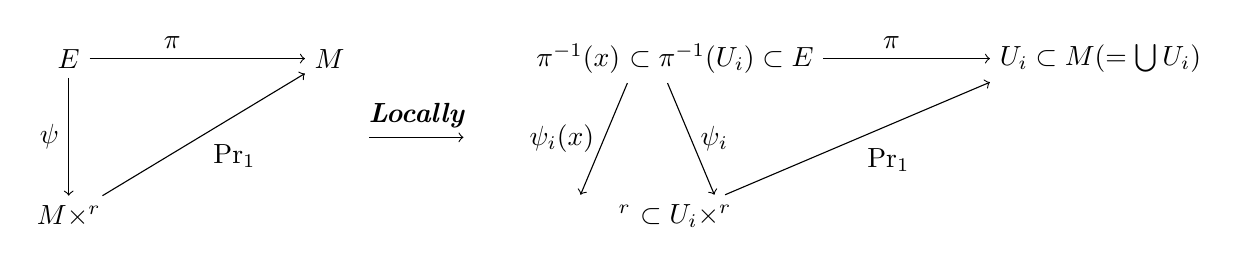
\begin{tikzpicture}
  \node (a1) at (90:1cm) {$E$};
  \node (a2) at (270:1cm) {$M\times \bC^r$};
  \node[right] (a3) at ([xshift=3cm]a1) {$M$};
  \draw[->] (a1) --node[left] {$\psi$} (a2) ;
  \draw[->] (a2) --node[below right] {$\mathrm{Pr}_1$} (a3) ;
  \draw[->] (a1) --node[above right,pos=0.3] {$\pi$} (a3) ;
  %%
  \coordinate (c) at ([,xshift=0.5cm,yshift=-1cm]a3);
  \draw[->] (c) --node[above,font=\bfseries\itshape] {Locally} ++(1.2cm,0);
  %%
  \node (b1) at ([xshift=7.7cm]a1) {$\pi^{-1}(x)$ $\subset \pi^{-1}(U_i)\subset E$};
  \node (b2) at ([xshift=7.7cm]a2) {$\bC^r$ $ \subset U_i \times \bC^r$};
  \node[right] (b3) at ([xshift=4cm]b1) {$U_i\subset M (=\bigcup U_i)$};
  \draw[->] ([xshift=1.28cm]b1.south west) --node[left] {$\psi_i (x)$} ([xshift=-1.2cm]b2.north) ;
  \draw[->] ([xshift=-1.98cm]b1.south east) --node[right] {$\psi_i$} ([xshift=0.5cm]b2.north) ;
  \draw[->] (b2) --node[below right] {$\mathrm{Pr}_1$} (b3.south west) ;
  \draw[->] (b1) --node[above right,pos=0.3] {$\pi$} (b3) ;
\end{tikzpicture}
\caption{The structure of the holomorphic vector bundle.}
\label{fig: vector bundle's structure}
\end{figure}

A \textit{holomorphic line bundle} is a holomorphic vector bundle of rank one.

Note that in the above definition the induced transition functions
\begin{align*}
\psi_{i j}(x):=\left(\psi_i \circ \psi_j^{-1}\right)(x): \mathbb{C}^r \longrightarrow \mathbb{C}^r
\end{align*}
are $\mathbb{C}$-linear for all $x \in U_i \cap U_j$.

Let $\pi_E: E \rightarrow X$ and $\pi_F: F \rightarrow X$ be two holomorphic vector bundles. A vector bundle homomorphism from $E$ to $F$ is a holomorphic map $\varphi: E \rightarrow F$ with $\pi_E=\pi_F \circ \varphi$ such that the induced map $\varphi(x): E(x) \rightarrow F(x)$ is linear with $\operatorname{rk}(\varphi(x))$ independent of $x \in X$. Two vector bundles $E$ and $F$ are isomorphic if there exists a bijective vector bundle homomorphism $\varphi: E \rightarrow F$.

{\normalem
Analogously to differential real or complex vector bundles, \emph{a holomorphic rank $r$ vector bundle $\pi\colon E\to X$ is determined by the holomorphic \textbf{\color{purple} cocycle} $\{(U_i, \, \psi_{ij}\colon U_i\cap U_j \to \operatorname{Gl}(r,\bC))\}$\footnote{$\operatorname{Gl}(r,\bC)$ represents the general linear group of complex matrixes of rank $r$.}.}}

\begin{definition}[][cocycle][def: cocycle]
  A cocycle is a closed cochain.
\end{definition}

\chapter{Sheaves and Cohomology}
\section{Origins: The Mittag-Leffler Problem}
\begin{fancybox}
  \textbf{The Mittag-Leffler Problem} :  Given a discrete  set $\{p_n\}$ of points in $S$ and a \textit{principal part} at $p_n$ for each $n$, does there exists such a meromorphic function $f$ on $S$ s.t. $f$ is holomorphic on $S$ up to $\{p_n\}$ and its \textit{principal part} at each $\{p_n\}$ is just the one given above?
\end{fancybox}
There are two approaches, both of which lead to \textbf{cohomology theories}. 

\section{Singular Cohomology}
Singular cohomology is a powerful invariant in topology, associating a graded commutative ring with any topological space. Every continuous map $f \colon X \rightarrow Y$ determines a homomorphism from the cohomology ring of $Y$ to that of $X$; this puts strong restrictions on the possible maps from $X$ to $Y$. Unlike more subtle invariants such as homotopy groups, the cohomology ring tends to be computable in practice for spaces of interest.
For a topological space $X$, the definition of singular cohomology starts with the singular chain complex:
\begin{align*}
\cdots \rightarrow C_{i+1} \stackrel{\partial_{i+1}}{\rightarrow} C_i \stackrel{\partial_i}{\rightarrow} C_{i-1} \rightarrow \cdots
\end{align*}
By definition, \textit{the singular homology of $X$ is the homology of this chain complex (the kernel of one homomorphism modulo is the image of the previous one).} In more detail, $C_i$ is the free abelian group on the set of continuous maps from the standard $i$-simplex to $X$ (called ``singular $i$-simplices in $X$ "), and $\partial_i$ is the $i$-th boundary homomorphism. The groups $C_i$ are zero for $i$ negative.
Now fix an abelian group $A$, and replace each group $C_i$ by its dual group $C_i^*:=\operatorname{Hom}\left(C_i, A\right)$, and $\partial_i$ by its dual homomorphism
\begin{align*}
d_{i-1}: C_{i-1}^* \rightarrow C_i^*.
\end{align*}
This has the effect of ``reversing all the arrows" of the original complex, leaving a cochain complex
\begin{align*}
\cdots \leftarrow C_{i+1}^* \stackrel{d_i}{\leftarrow} C_i^* \stackrel{d_{i-1}}{\leftarrow} C_{i-1}^* \leftarrow \cdots
\end{align*}
For an integer $i$, the $i^{\text {th }}$ cohomology group of $X$ with coefficients in $A$ is defined to be $\operatorname{ker}\left(d_i\right) /$ im $\left(d_{i-1}\right)$ and denoted by $H^i(X, A)$. The group $H^i(X, A)$ is zero for $i$ negative. The elements of $C_i^*$ are called singular $i$-cochains with coefficients in $A$. (Equivalently, an $i$-cochain on $X$ can be identified with a function from the set of singular $i$-simplices in $X$ to A.) Elements of $\operatorname{ker}(d)$ and $\operatorname{im}(d)$ are called cocycles and coboundaries, respectively, while elements of $\operatorname{ker}(d) / \operatorname{im}(d)=H^i(X, A)$ are called cohomology classes (because they are equivalence classes of cocycles).

In what follows, the coefficient group $A$ is sometimes not written. It is common to take $A$ to be a commutative ring $R$; then the cohomology groups are $R$-modules. A standard choice is the ring $\mathbf{Z}$ of integers.
Some of the formal properties of cohomology are only minor variants of the properties of homology:
\begin{itemize}
  \item A continuous map $f: X \rightarrow Y$ determines a pushforward homomorphism $f_*\colon H_i(X) \rightarrow H_i(Y)$ on homology and a pullback homomorphism $f^*\colon H^i(Y) \rightarrow H^i(X)$ on cohomology. This makes cohomology into a contravariant functor from topological spaces to abelian groups (or $R$-modules).
  \item Two homotopic maps from $X$ to $Y$ induce the same homomorphism on cohomology (just as on homology).
  \item The Mayer-Vietoris sequence is an important computational tool in cohomology, as in homology. Note that the boundary homomorphism increases (rather than decreases) degree in cohomology. That is, if a space $X$ is the union of open subsets $U$ and $V$, then there is a long exact sequence:
  \begin{align*}
  \cdots \rightarrow H^i(X) \rightarrow H^i(U) \oplus H^i(V) \rightarrow H^i(U \cap V) \rightarrow H^{i+1}(X) \rightarrow \cdots
  \end{align*}
  \item There are relative cohomology groups $H^i(X, Y ; A)$ for any subspace $Y$ of a space $X$. They are related to the usual cohomology groups by a long exact sequence:
  \begin{align*}
  \cdots \rightarrow H^i(X, Y) \rightarrow H^i(X) \rightarrow H^i(Y) \rightarrow H^{i+1}(X, Y) \rightarrow \cdots
  \end{align*}
  \item The universal coefficient theorem describes cohomology in terms of homology, using Ext groups. Namely, there is a short exact sequence
  \begin{align*}
  0 \rightarrow \operatorname{Ext}_{\mathbb{Z}}^1\left(\mathrm{H}_{i-1}(X, \mathbb{Z}), A\right) \rightarrow H^i(X, A) \rightarrow \operatorname{Hom}_{\mathbb{Z}}\left(H_i(X, \mathbb{Z}), A\right) \rightarrow 0
  \end{align*}
  A related statement is that for a field $F, H^i(X, F)$ is precisely the dual space of the vector space $H_i(X, F)$.
  \item If $X$ is a topological manifold or a CW complex, then the cohomology groups $H^i(X, A)$ are zero for $i$ greater than the dimension of $X$. If $X$ is a compact manifold (possibly with boundary), or a CW complex with finitely many cells in each dimension, and $R$ is a commutative Noetherian ring, then the $R$-module $H^i(X, R)$ is finitely generated for each $i$.
\end{itemize}

  On the other hand, cohomology has a crucial structure that homology does not: for any topological space $X$ and commutative ring $R$, there is a bilinear map, called the cup product:
  \begin{align*}
  H^i(X, R) \times H^j(X, R) \rightarrow H^{i+j}(X, R)
  \end{align*}
  defined by an explicit formula on singular cochains. The product of cohomology classes $u$ and $v$ is written as $u \cup v$ or simply as $u v$. This product makes the direct sum
  \begin{align*}
  H^*(X, R)=\bigoplus_i H^i(X, R)
  \end{align*}
  into a graded ring, called the cohomology ring of $X$. It is graded-commutative in the sense that:
  \begin{align*}
  u v=(-1)^{i j} v u, \quad u \in H^i(X, R), v \in H^j(X, R)
  \end{align*}
  For any continuous map $f: X \rightarrow Y$, the pullback $f^*: H^*(Y, R) \rightarrow H^*(X, R)$ is a homomorphism of graded $R$-algebras. It follows that if two spaces are homotopy equivalent, then their cohomology rings are isomorphic.
  
  Here are some of the geometric interpretations of the cup product. In what follows, manifolds are understood to be without boundary, unless stated otherwise. A closed manifold means a compact manifold (without boundary), whereas a closed submanifold $N$ of a manifold $M$ means a submanifold that is a closed subset of $M$, not necessarily compact (although $N$ is automatically compact if $M$ is).
  \begin{itemize}
  \item Let $X$ be a closed oriented manifold of dimension $n$. Then Poincaré duality gives an isomorphism $H^i X \cong H_{n-i} X$. As a result, a closed oriented submanifold $S$ of codimension $i$ in $X$ determines a cohomology class in $H^X X$, called [S]. In these terms, the cup product describes the intersection of submanifolds. Namely, if $S$ and $T$ are submanifolds of codimension $i$ and $j$ that intersect transversely, then
  \begin{align*}
  [S][T]=[S \cap T] \in H^{i+j}(X)
  \end{align*}
  where the intersection $S \cap T$ is a submanifold of codimension $i+j$, with an orientation determined by the orientations of $S, T$, and $X$. In the case of smooth manifolds, if $S$ and $T$ do not intersect transversely, this formula can still be used to compute the cup product $S\cap T$, by perturbing $S$ or $T$ to make the intersection transverse.
  
  More generally, without assuming that $X$ has an orientation, a closed submanifold of $X$ with an orientation on its normal bundle determines a cohomology class $X$ is a noncompact manifold, then a closed submanifold (not necessarily compact) determines a cohomology class on $X$. In both cases, the cup product can again be described in terms of intersections of submanifolds.
  
  Note that Thom constructed an integral cohomology class of degree $7$ on a smooth $14$-manifold that is not the class of any smooth submanifold. On the other hand, he showed that every integral cohomology class of positive degree on a smooth manifold has a positive multiple that is the class of a smooth submanifold. Also, every integral cohomology class on a manifold can be represented by a ``pseudomanifold", that is, a simplicial complex that is a manifold outside a closed subset of codimension at least $2$.
  \item For a smooth manifold $X$, de Rham's theorem says that the singular cohomology of $X$ with real coefficients is isomorphic to the de Rham cohomology of $X$, defined using differential forms. The cup product corresponds to the product of differential forms. This interpretation has the advantage that the product on differential forms is graded commutative, whereas the product on singular cochains is only graded-commutative up to chain homotopy. In fact, it is impossible to modify the definition of singular cochains with coefficients in the integers $\mathbb{Z}$ or in $\mathbb{Z} / p$ for a prime number $p$ to make the product graded-commutative on the nose. The failure of graded-commutativity at the cochain level leads to the Steenrod operations on $\bmod p$ cohomology.
\end{itemize}

  Very informally, for any topological space $X$, elements of $H^i(X)$ can be thought of as represented by codimension- $i$ subspaces of $X$ that can move freely on $X$. Forampe one way to define an element of $H^i(X)$ is to give a continuous map ffrom $X$ to a manifold $M$ and a closed codimension-i submanifold $N$ of $M$ with an orientation on the normal bundle. Informally, one thinks of the resulting class $f^*([N]) \in H^i(X)$ as lying on the subspace $f^{-1}(N)$ of $X$; this is justified in that the class $f^*([N])$ restricts to zero in the cohomology of the open subset $X-f^{-1}(N)$. The cohomology class $f^*([N])$ can move freely on $X$ in the sense that $N$ could be replaced by any continuous deformation of $N$ inside $M$.














